\section{Zoom Video Conferencing Behaviour}
From the captured dataset we have infered the behaviour of the Zoom application, as a function of different channel conditions. We chose as the limittting parameter the bandwidth of the channel, as it is the easy to control, and also the easiest to interpret.
% While capturing the dataset of Zoom conferencing traffic samples, we have investigated Zoom behavior when exposed to varying channel bandwidth conditions. It is logical to assume that bandwidth transition periods will impact video quality and will reflect on users' perceived quality. Therefore, it is advantageous to understand the impact of these transitions on traffic features and labels.

\subsection{Impact of reduced available bandwidth}
We shall refer to 'transition' as the period during which the Zoom application adjusts its video transmission parameters when a degradation is introduced to the channel quality, such as a drop of bandwidth for example. We discovered that during transition, Zoom goes through the following cycle: (1) reducing video spatial resolution; (2) reducing frames per second (fps); and (3) restoring spatial resolution to original with lower fps. We observed that such a transition can typically take up to 10 sec, at the end of which the video spatial resolution is restored to the original value while a lower fps is used to compensate for the reduced available bandwidth. This behavior makes sense, given that in typical video conferencing scenario there are only small spatial movements and therefore users' perceived quality will be impacted more by the spatial resolution than by the temporal resolution. The charts of \Cref{fig:adapt-patt} illustrate the steady state variation of fps and latency as a function of available bandwidth (measured after waiting for the transition period to pass and the spatial resolution to be restored). They were taken from a single session; however, they represent a consistent behavior that we have observed in multiple similar sessions. A dramatic drop from 25 fps to less than 10 fps is observed when the available bandwidth drops from 120 kbps to 60 kbps. 
\subsection{Impact of reduced bandwidth on Quantization Parameter (Qp)}
Assuming that Qp may be used by Zoom as a dominant parameter to adapt to changing channel bandwidth conditions, and therefore may be used as a good indicator for QoE, we have explored the change of Qp when reducing the available bandwidth. We observed that the Qp remains unchanged for I-frames and is slightly decreased with reduced bandwidth for P-Frames. This indicates that the Zoom application tries to compensate for the reduced bandwidth, which is accommodated by reduced fps, by adjusting to finer quantization of the P-Frames, however, the change is small, and we consider it too hard to estimate from encrypted traffic. Therefore, it is less valuable as QoE predictor. The change of Qp with the reduced bandwidth is illustrated in \Cref{fig:qp-change}.

\begin{figure}
    \centering
    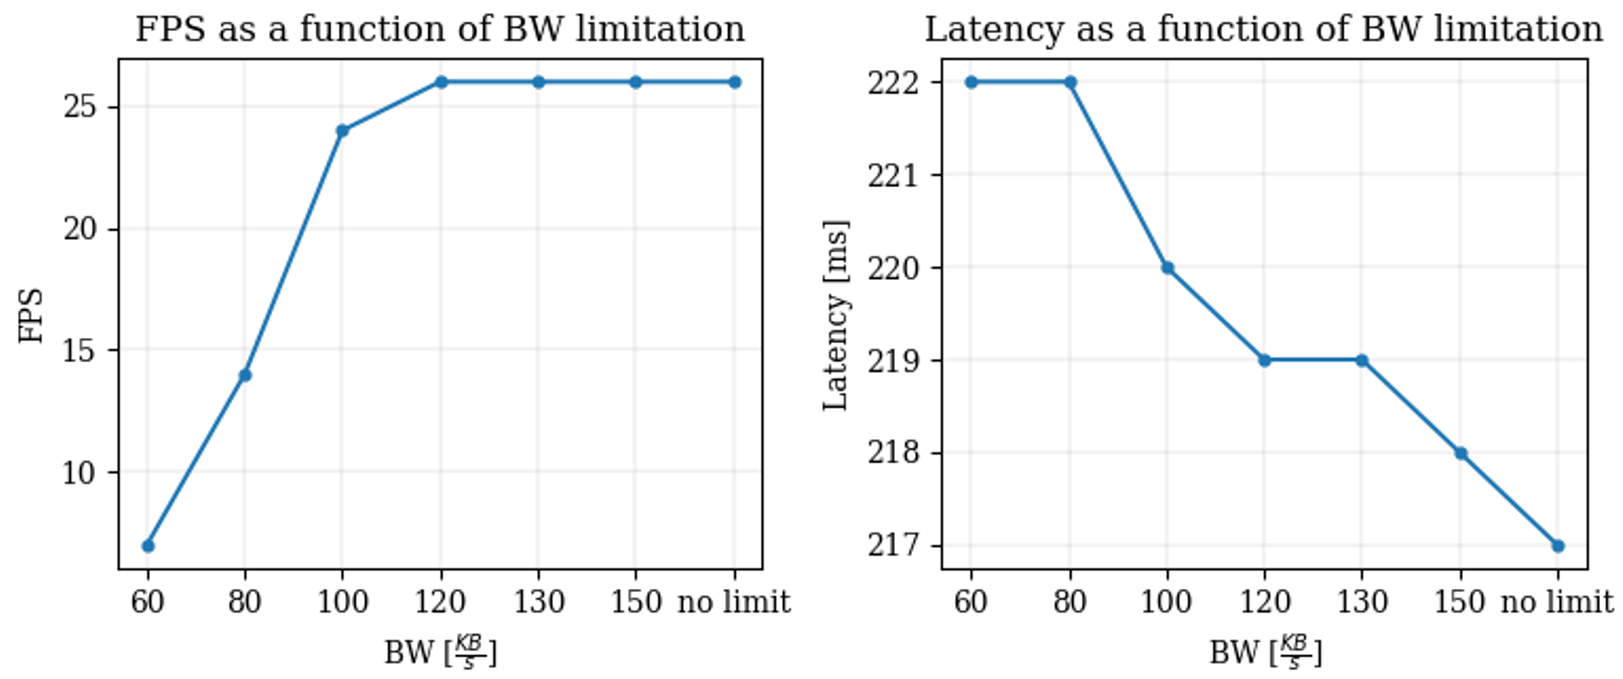
\includegraphics[scale=0.18]{adapt_patt.png}
    \caption{Zoom adaptation patterns to dropping bandwidth}
    \label{fig:adapt-patt}
\end{figure}

\begin{figure}
    \centering
    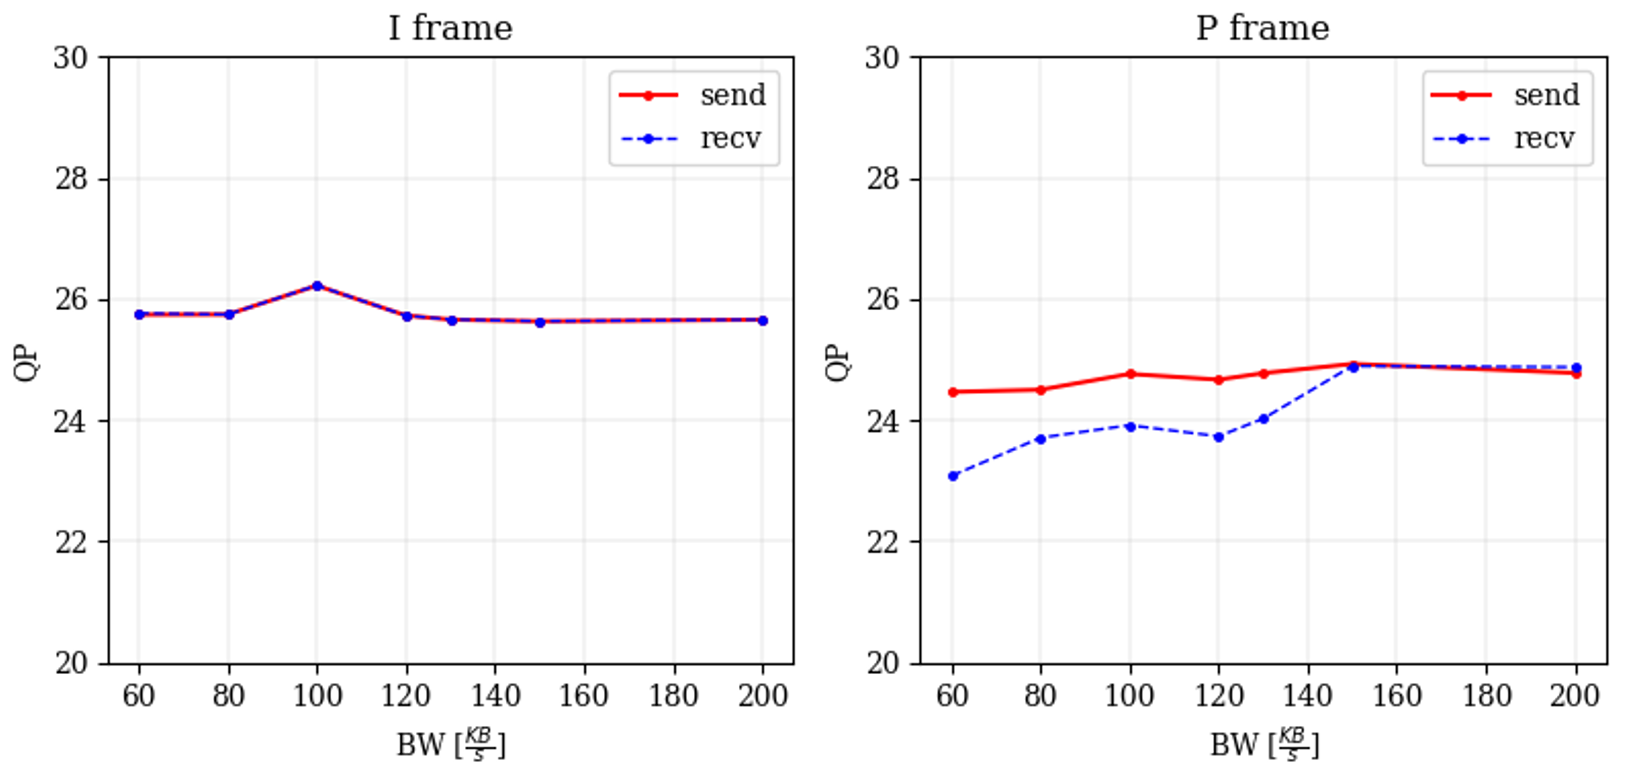
\includegraphics[scale=0.18]{Qp_to_bw.png}
    \caption{Zoom Qp change as a function of dropping bandwidth}
    \label{fig:qp-change}
\end{figure}

% \subsection{Full Reference (FR) QoE metrics}
% We extracted several Full Reference video quality metrics from Zoom traffic. In order to assess the quality degradation caused by reduced bandwidths, we needed to compare a reference source video of original quality to the same video stream at the receiving end, that was impacted by the network conditions. We have access to the video that is recorded by the Zoom application. We observed that when establishing a 2-party conference call, Zoom reduces the quality of the recoded video at the source and at the destination at the same time. In order to obtain a good quality reference, we managed to force the Zoom application to produce and record a good quality video. This was accomplished by adding to the call a 3rd party without a bandwidth limitation. This way the sending Zoom application allows to record a good quality reference which is not impacted by the restricted bandwidth of the 2nd party to the call. The setup used to record the reference and the destination videos is depicted in \Cref{fig:vmaf-setup}. In order to perform a reasonably accurate comparison between the 2 recorded streams, they have to be synchronized. We used the audio recording to synchronize the streams by creating an abrupt loud instantaneous noise (similar to "cut" used in recording a movie "video take") and synchronized the videos at the sender and recipient ends using that noise.
% The results of the Full reference video QoE metrics measured using the setup depicted in \Cref{fig:vmaf-setup} are provided in \Cref{fig:qual-metrics}. The slight improvement of quality observed when the bandwidth is decreased can be explained by the slight decrease of the Qp parameter performed by Zoom during the bandwidth drop transition period (depicted in \Cref{fig:adapt-patt}). It is assumed that Zoom decreases the Qp to compensate for reduced quality during the bandwidth drop transition.

\begin{figure}
    \centering
    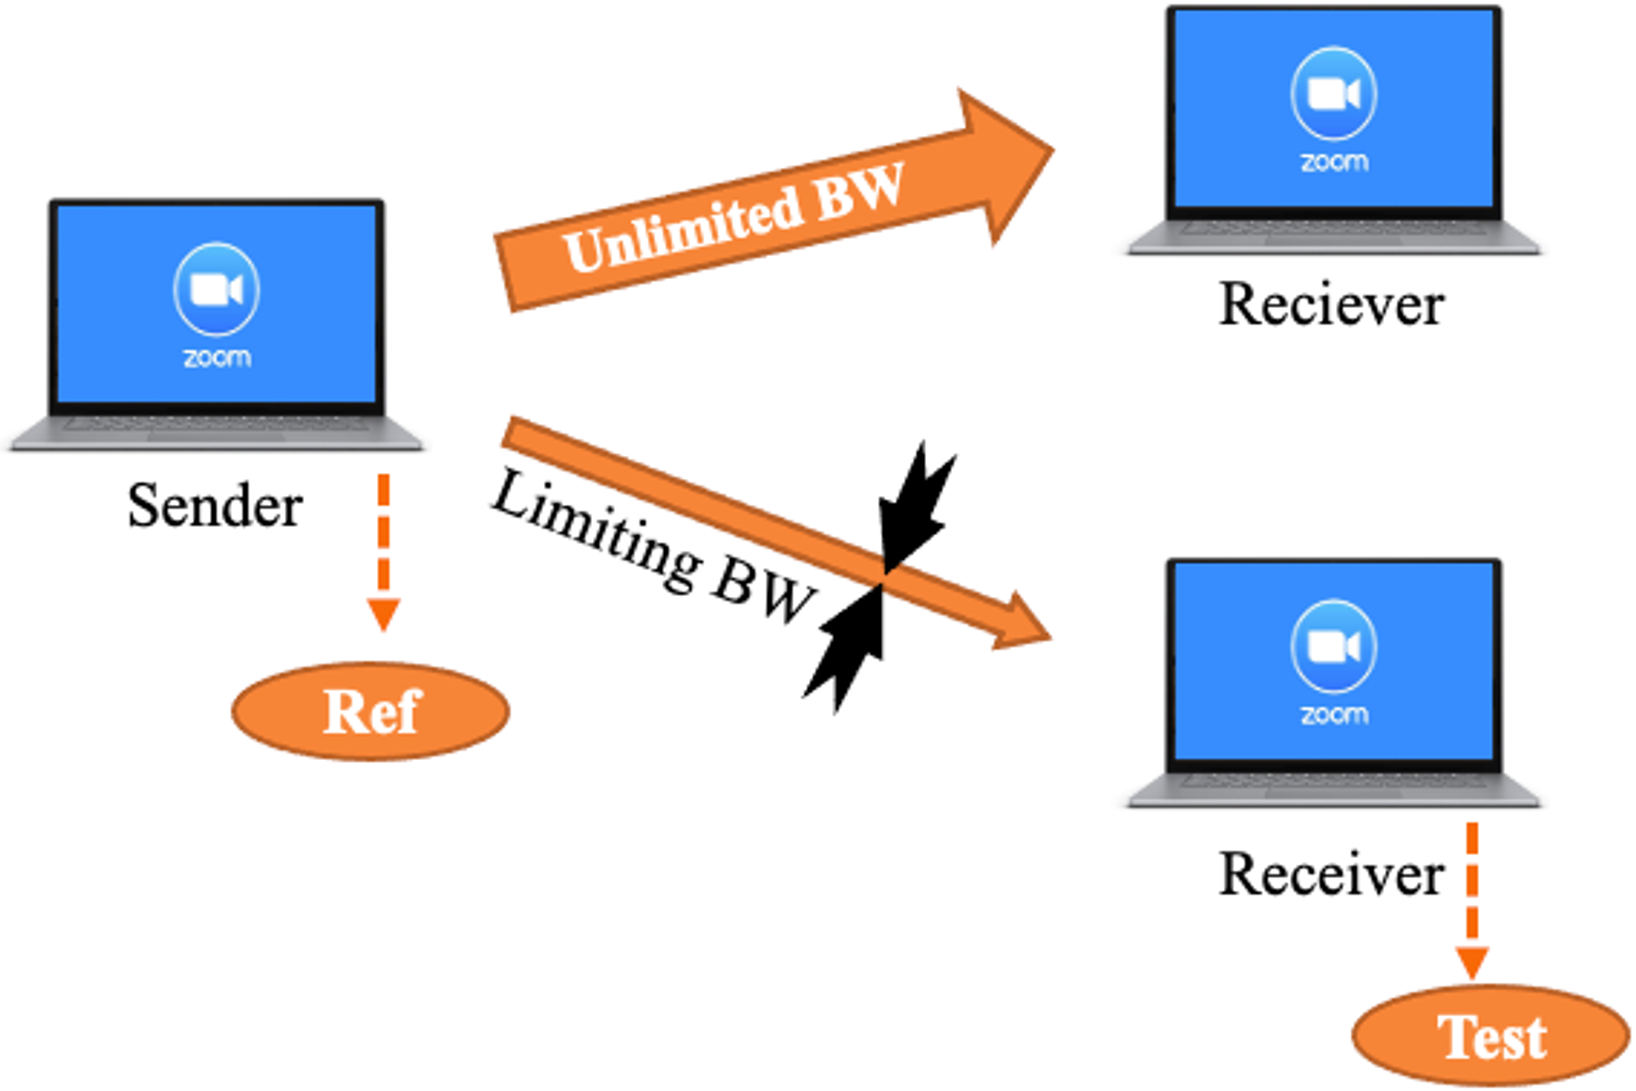
\includegraphics[scale=0.18]{vmaf_setup.png}
    \caption{VMAF full reference Zoom testing setup}
    \label{fig:vmaf-setup}
\end{figure}

\begin{figure}
    \centering
    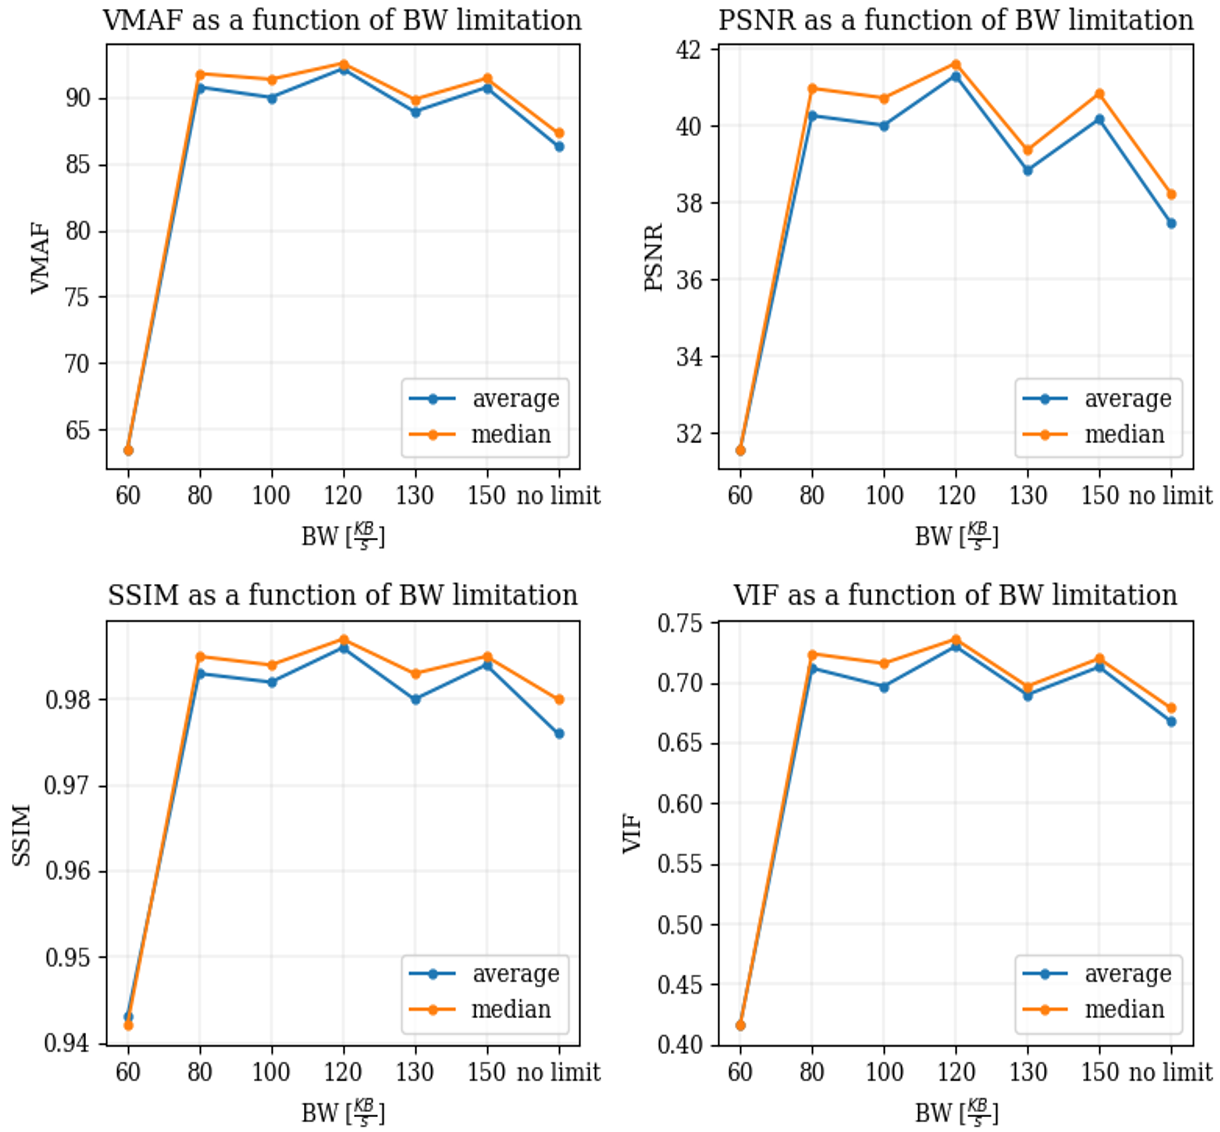
\includegraphics[scale=0.25]{vmaf_to_bw.png}
    \caption{Measured Zoom quality metrics as a function of dropping bandwidth}
    \label{fig:qual-metrics}
\end{figure}


% \subsection{NIQE – NR quality metric}
% Due to the challenges of recording Zoom video sessions with FR and in order to make the dataset more accommodating to future expansions (which do not necessitate complicate setups and saving of a refence for each recorded video clip), we researched the No Reference (NR) QoE metric alternatives. A promising NR metric that has emerged is the Naturalness Image Quality Evaluator (NIQE) \cite{mittal2012making}, which measures the distance of the frame from naturalness, therefore, a smaller score indicates better perceptual quality. NIQE measures the distance between the Natural Scene Statistics (NSS)-based features calculated from an image to the features obtained from an image database used to train the model. The features are modeled as multidimensional Gaussian distributions. We calculated NIQE as a function of bandwidth, resolution and fps. The corresponding graphs are depicted in \Cref{fig:niqe-fps-bw-res}. As can be seen in \Cref{fig:niqe-fps-bw-res} (b) and (c), the NIQE is consistent with available bandwidth and video frame resolution respectively, such that the larger the bandwidth or the resolution, the smaller the NIQE, thus indicating better quality.  We can observe a range of resolutions for which the NIQE value remains constant, indicating that the image naturalness metric at these resolutions is sufficiently good despite the change. An interesting observation is depicted in \Cref{fig:niqe-fps-bw-res} (a), indicating a change of NIQE with fps, whereas the metric is measured per single frame and is therefore spatial by nature. The temporal resolution of the video frames has an impact on the spatial quality. This is due to the compression algorithm that utilizes quantized residuals which are determined by block prediction accuracy, which is in turn impacted by the magnitude of the Motion Vectors (MV) used for Inter-prediction. The larger the movement between consecutive frames, the larger the MV magnitude and the less accurate is the prediction, thus increasing the value of the temporary predicted block residuals and reducing the quality due to their quantization.

\begin{figure}
    \centering
    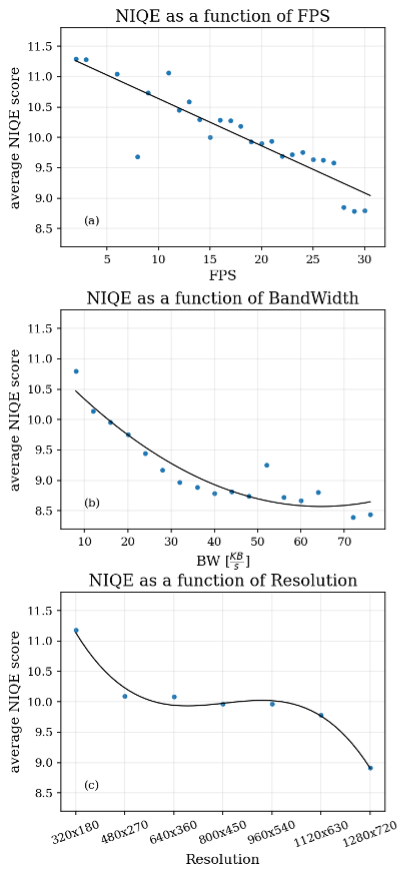
\includegraphics{niqe_to_fps.png}
    \caption{Measured Zoom NIQE quality metric as a function of fps, bandwidth, and resolution}
    \label{fig:niqe-fps-bw-res}
\end{figure}